\documentclass[11pt]{article}
\usepackage{lmodern}
\usepackage{amssymb,amsmath}
\usepackage{ifxetex,ifluatex}
%\usepackage{fixltx2e} % provides \textsubscript
\usepackage{xr} % referencing external ducument
\ifnum 0\ifxetex 1\fi\ifluatex 1\fi=0 % if pdftex
  \usepackage[T1]{fontenc}
  \usepackage[utf8]{inputenc}
\else % if luatex or xelatex
  \ifxetex
    \usepackage{mathspec}
  \else
    \usepackage{fontspec}
  \fi
  \defaultfontfeatures{Ligatures=TeX,Scale=MatchLowercase}
\fi
% use upquote if available, for straight quotes in verbatim environments
\IfFileExists{upquote.sty}{\usepackage{upquote}}{}
% use microtype if available
\IfFileExists{microtype.sty}{%
\usepackage{microtype}
\UseMicrotypeSet[protrusion]{basicmath} % disable protrusion for tt fontshttps://de.overleaf.com/project/5e85b0680d0bed00011ea790
}{}
\usepackage[margin=1in]{geometry}
\usepackage{hyperref}
\hypersetup{unicode=true,
            pdftitle={Title: Human Neandertal Admixture dating limits MBE Supplements},
            pdfauthor={Leonardo Nicola Martin Iasi (Max Planck Institute for Evolutionary Anthropology, MPI EVA), Dr.~Benjamin Marco Peter (MPI EVA, benjamin\_peter@eva.mpg.de)},
            pdfborder={0 0 0},
            breaklinks=true}
\urlstyle{same}  % don't use monospace font for urls
 
%\usepackage{natbib}
%\bibliographystyle{References/my_abbrvnat}
%\setcitestyle{authoryear,open={(},close={)}}

\usepackage{graphicx,grffile}
\makeatletter
\def\maxwidth{\ifdim\Gin@nat@width>\linewidth\linewidth\else\Gin@nat@width\fi}
\def\maxheight{\ifdim\Gin@nat@height>\textheight\textheight\else\Gin@nat@height\fi}
\makeatother
% Scale images if necessary, so that they will not overflow the page
% margins by default, and it is still possible to overwrite the defaults
% using explicit options in \includegraphics[width, height, ...]{}

\setkeys{Gin}{width=\maxwidth,height=\maxheight,keepaspectratio}
\IfFileExists{parskip.sty}{%
\usepackage{parskip}
}{% else
\setlength{\parindent}{0pt}
\setlength{\parskip}{6pt plus 2pt minus 1pt}
}
\setlength{\emergencystretch}{3em}  % prevent overfull lines
\providecommand{\tightlist}{%
  \setlength{\itemsep}{0pt}\setlength{\parskip}{0pt}}
\setcounter{secnumdepth}{0}
% Redefines (sub)paragraphs to behave more like sections
\ifx\paragraph\undefined\else
\let\oldparagraph\paragraph
\renewcommand{\paragraph}[1]{\oldparagraph{#1}\mbox{}}
\fi
\ifx\subparagraph\undefined\else
\let\oldsubparagraph\subparagraph
\renewcommand{\subparagraph}[1]{\oldsubparagraph{#1}\mbox{}}
\fi

\usepackage{setspace}
\onehalfspacing
\usepackage[left]{lineno}
\linenumbers
\usepackage[none]{hyphenat}
\usepackage{amsfonts}
\usepackage{amssymb}
\usepackage{graphicx}
\usepackage{float}
\usepackage{xcolor}

\floatplacement{figure}{H}
\begin{document}

\section{Reviewer 1}\label{Reviewer 1}

\paragraph{1.}
A key contribution that I would have hoped to get out of the manuscript is the power to reject the model of ``pulse admixture’’ given data simulated under a non-pulse model. To evaluate the power to detect a difference from $t_d$ = 1 (which is equivalent to the pulse model) in a likelihood-ratio test framework. This would assume a best-case scenario of no noise in the estimation of segment lengths, but would help inform the reader of the parameter regimes that are identifiable in the model. In my view this analysis is essential because it provides statistical evidence for how seriously I should take the claims made in the real data analysis.

\paragraph{Answer to 1.1}
We included a best case scenario as the first part of the results. Here we simulate perfectly known segments under the extended pulse with multiple durations of gene flow and a mean time of gene flow at 1500 generations ago. We fitted the simple and extended pulse to it and performed a likelihood ratio test. The result is depicted in the result figure x. 

\paragraph{2.}
A secondary question that is analytically tractable is how the power described above is shaped by the time-since admixture ($t_m$), which is implied by the statements that requiring samples closer to the time of admixture would be helpful for future inference (line 20 in the abstract for example). This would be useful to quantify what kind of data might be necessary to reject the model of pulse admixture (or if it is even possible at all with current human data parameters?). As this is a claim vaguely made in the paper – I believe that a statistical evaluation of the power to reject the pulse model with data from different time-points post-admixture. 

\paragraph{Answer to 1.2}
Figure x in the results also depicts the likelihood ratio between the simple and extended pulse for segments sampled 50 generation after the end of the respective gene flow. 

\paragraph{3.}
Is there a difference in the power to reject the “pulse model” if one uses ALD at different length scales or realized segments? This would place clearer value on one summary statistic over the other for pursuing further inference in aDNA datasets. 

\paragraph{Answer to 1.3}
We compared the performance for multiple durations of gene flow with a mean time of 1500 generations ago from msprime simulations using the decay of ancestry LD with perfectly known recombination distances.


\paragraph{4.}
The focus in the paper is to distinguish between models of an extended duration of admixture using the decay of “admixture LD” but little attention is paid to the model using segments, although the authors detail this in the derivations first. The admixture LD is easier to calculate from data to avoid haplotype phasing, but in theory segments are detectable (Skov et al 2018). In the simulations detailed using msprime (Kellher et al 2016), it should be possible to directly use the introgressed segments for this task as well. In my view the authors should either entirely describe the results in terms of ALD, and making this more explicit in the section on Results/Simulations to say that this is the specific summary statistic that is presented throughout the results or to include supplementary results where the summary statistic of admixture segment lengths are used as well. 

\paragraph{Answer to 1.4}
We 

\subsection{Minor Comments}\label{Minor Comments}

Page 2 – line 52: avoid starting a sentence with “It” as it obscures the subject of the sentence, I think a more appropriate start would be “Uncertainty in the timing of gene flow also would affect …”

\bold{Answer:} we changed it to "More certainty in the timing of gene flow also would affect  assumptions about introgressed allele frequencies and their distribution in present-day human genomes and conclusions drawn about the phenotypic effects and selective pressures of introduced alleles."

There is an error in notation on page 11- line 3: should be “tm” instead of “td” I believe.

\bold{Answer:} changed to "td"

A typo in the caption for Table S1: “standart” vs. “standard”

\bold{Answer:} changed to "standard"

A suggestion on the formatting for Table S2 would be to include the model estimates as the columns (and the different scenarios as rows), and the confidence intervals as part of the entries for the estimates in brackets / parentheses. The reader should be able to readily compare the same parameter across these fits by just looking at a single column. 

\bold{Answer:} the table format was changed as suggested and can be found in the supplements as table 2.

There are several comments with regards to the structure and layout of the provided software code:

Improve documentation for the `fit-extended-pulse` and `fit-simple-pulse` functions to better describe the inputs. I would recommend using the `roxygen` formatting for documentation to make the code more readable and useable. 
One suggestion would be to provide an example input for these functions within the repository to help the end user understand more clearly the required data table format. 
I would suggest a “requirements.md” or “requirements.txt” file in the main directory of the code to inform the user of the libraries required to import (and their versions if possible).

\section{Reviewer 2}\label{Reviewer 2}

\paragraph{1.}
My main concern relates to the “Application to Neandertal data.” My understanding of the manuscript title (An extended admixture pulse model reveals the limits to the dating of Human-Neandertal introgression) is that the extended model provides the limits (or bounds) for the dating of introgression. I do not think that this manuscript shows that. Instead, it seems like the application to Neandertal data shows that there is little power to differentiate tested scenarios (with varying gene flow durations). Perhaps the word “limits” in the title refers to the *limitations* of the model? I would like to hear from the authors about their intent and, if my understanding of the title is correct (i.e., limits == bounds), then I would like to see a more detailed discussion about this issue in the manuscript see comments below.

\paragraph{Answer to 2.1}

\paragraph{2.}
Overall, I think this subsection of Results is a bit underwhelming and somewhat disconnected from the part where authors examine their model with simulations. Given how the problem is introduced and the manuscript is presented, I would expect a more thorough examination of both the duration and mean time of Neandertal-human introgression. I think it is worth mentioning in the “Application to Neandertal data” section what are the estimates for the mean time of admixture and how they compare with published data. I understand this has been reported in previous studies, but I believe it would be important to report the estimates using their methods in a paper like this.

\paragraph{Answer to 2.2}

\paragraph{3.}
I would also like to hear from the authors the reasons why the specific scenarios were chosen for the simulations. Since the paper focuses on Neandertal-Human introgression and the range for the dating of this event is well known (37-86kya, 41-54kya, or 50-60kya as reported by the authors), then I would expect the simulations to cover this range. Perhaps I missed something, but the simulated scenarios seem to include mostly very recent dates for introgression. The few examples where mean time of admixture match what is known for the Neandertal-Human introgression use the same duration of gene flow (800 generations). How does the inference work for shorter durations? It would be great to see with simulations if the estimates for the duration of admixture are robust for an admixture time that matches the expected range for Neanderthal introgression. Perhaps the application to the data does that already, but still, it is good to see how good the inferences for plausible scenarios are especially considering different admixture durations.

\paragraph{Answer to 2.3}
We included more simulations on different admixture durations with a mean time of 1500 generations ago (close to the time estimated for the Neandertal-Human admixture). Simulation used a constant recombination rate. 

\paragraph{4.}
Generally speaking, I miss some discussion about the applicability of this model to the study of other events in human history/evolution and beyond humans.

\paragraph{Answer to 2.4}

\subsection{Minor Comments}\label{Minor Comments}

Minor comments:
Consider adding “on average” to the first sentence of the abstract (referring to the percentage of Neandertal DNA).

\bold{Answer:} changed to "Neandertal DNA makes up 2-3\% of the genomes of all non-African individuals on average."

Page 6, line 20. “Ti represents the time when segment Li entered the population” Would it be segment i instead of Li? 

\bold{Answer:}

Page 10, first line. Is it supposed to be tm=500 instead of td=500?

\textbf{Answer:} changed to "(i.e. if $t_m= 500$ generations, then $t_d = 250$ and most gene flow occurs between  375 and 625
generations ago)."


I do not follow what is described on page 13, first and second paragraphs. Would it be left panels instead of right? If that’s the case, then I can see that for panel C, not for panel A. If my reasoning is correct, then also change the reference to the right panels (not left) in the next paragraph.

\textbf{Answer:} 

Page 12, line 56: I believe this is supposed to be Figure 4A. 

\textbf{Answer:} changed to "Figure 4A"

Typo? page 18, line 40/41 The effective… *and are* based on estimates…” 

\textbf{Answer:} changed to "are"

Figure 2, panel A: Please use “Single pulse” instead of “Pulse.”

\textbf{Answer:} changed to "simple pulse"


Figure 2, panel B: It seems like the color legend is redundant. Admixture duration is shown at the bottom of each column already, so no need to use the different colors. Also, it could be a bit distracting since you use the same colors for Figure 4. 

\textbf{Answer:} The figure is updated and the colores are changed.

Figure 3: why only the second dot is green?

\textbf{Answer:} The second dot is the one for the effect size of the gene flow model to easier compare it since the gene flow model is the main concern of the paper.

Add units for time in figure 4. I suppose it is generations.

\textbf{Answer:} 

References to supplementary figures lack the word “Figure.” 

\textbf{Answer:} "Figure" was added.

\section{Reviewer 3}\label{Reviewer 3}

\paragraph{1.}
As shown in their figures, the current version of this method is a biased method. Therefore, the single major concern I have about their paper is that it lacks explanations and investigations on the bias and variance of this newly proposed method. Hence some improvements are needed. In particular, why is it a biased method, and is it possible to improve on it further?

\paragraph{Answer to 3.1}

\paragraph{2.}
Simulation: the basic version of msPrime does not shine at simulating long-range LD in recent generations, and therefore it was recommended, when long-range correlations are used, the msPrime with Wright-Fisher extension should be used instead to overcome the biases in especially the recent time scale (see Nelson et al. 2020, PLoS genetics). When the admixture duration is long and extends to very recent time as in some of the simulations for the extended pulse model, and long-range information (LD, segment length) is used in inference, it might be essential to incorporate the WF extension in the simulation.Some of the biases perhaps would disappear with better simulation. It is also possible that a more realistic simulation would lead to even larger bias, which would also be essential to know.

\paragraph{Answer to 3.2}

\begin{figure}
\centering
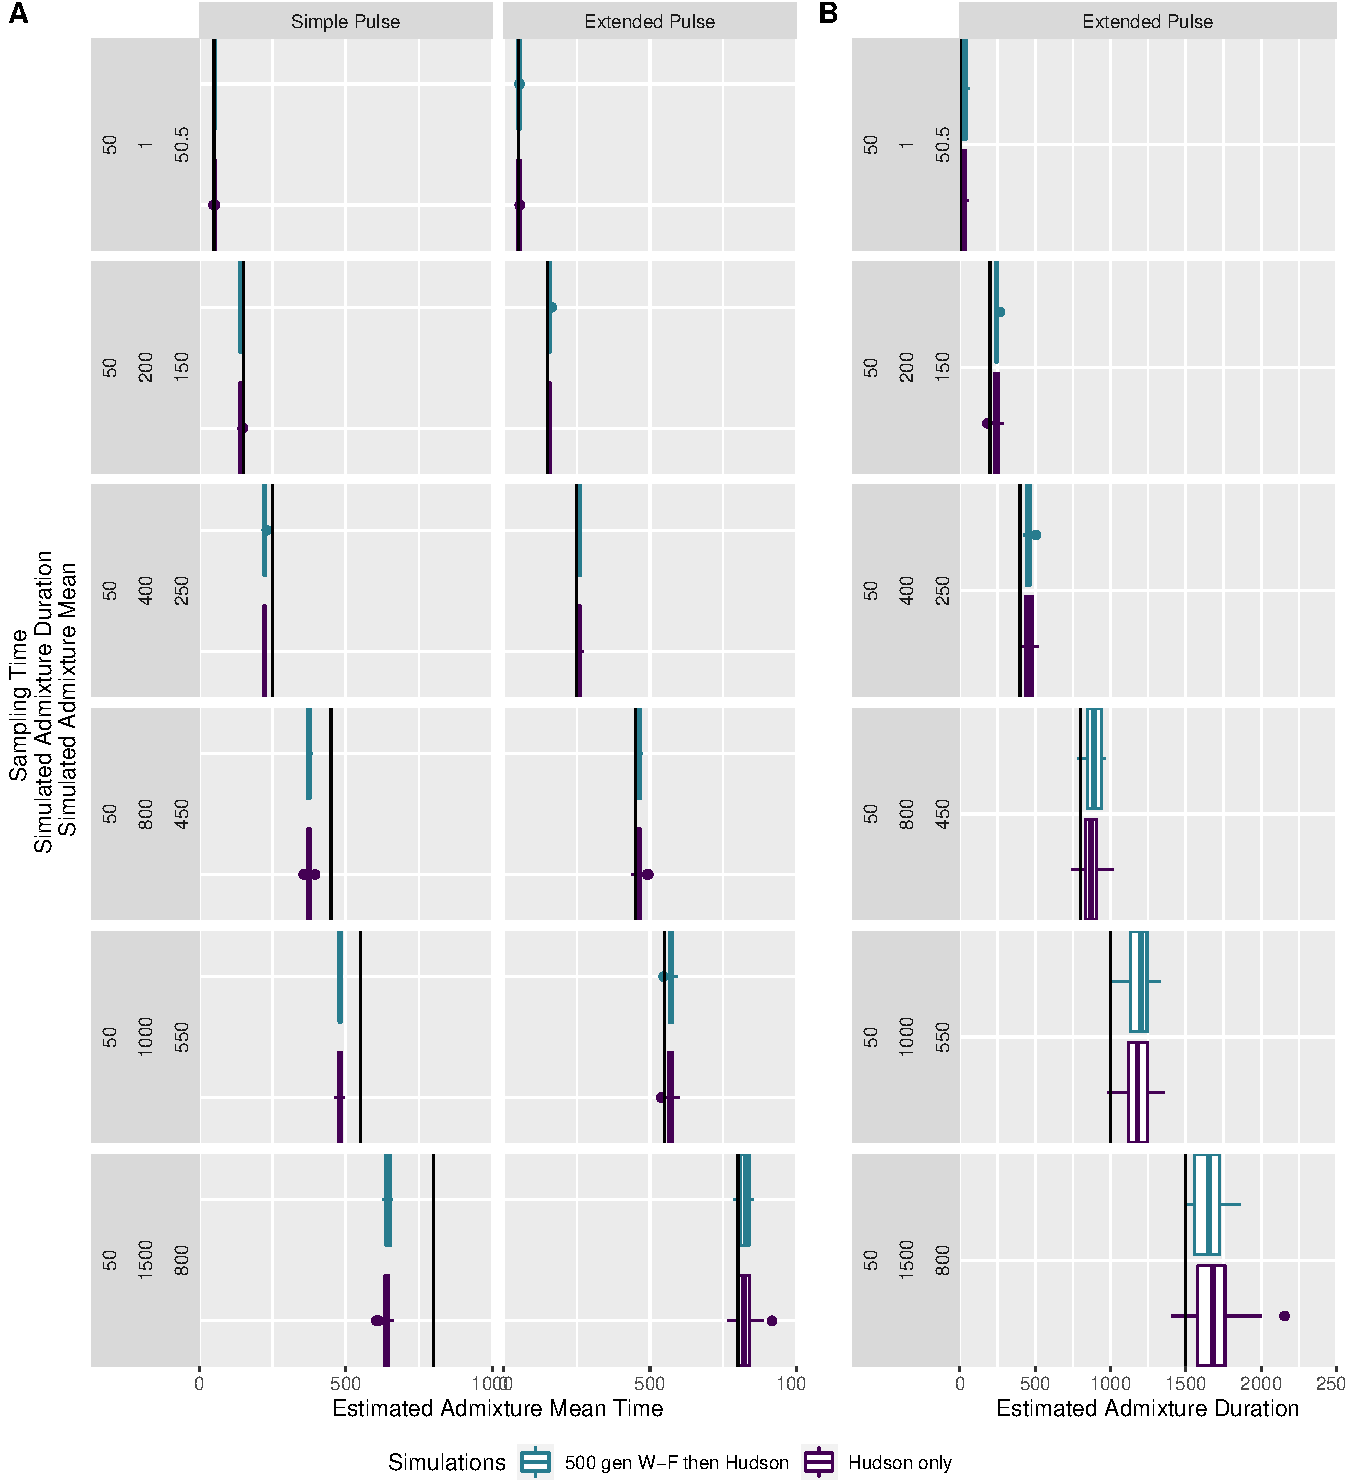
\includegraphics[width=16cm,height=18cm,keepaspectratio]{ATE_Revisions_files/figure-latex/figR4-1.pdf}
\caption{\label{fig:fig_R} }
\end{figure}

\paragraph{3.}
Model: I wonder if the authors decided to dismiss the admixture fraction too soon without giving enough justifications (on page 8 line 24-24). While this assumption that recombination within archaic segments can be ignored is perhaps justifiable in some previous work, this paper works on a more delicate problem, and subtle signals and biases matter more. To differentiate single pulse and extended pulse, fixed admixture fraction in a single pulse and increasing admixture fraction over time in the extended pulse is a signature of these different admixture models. I wonder if some of the biases in their method is related to this simplification. To elaborate, let’s assume total admixture fraction is $\alpha$, and recombination rate r, mean time of admixture T, under a single pulse model, the effective recombination rate which will affect the introgressed segment length with rate $(1-\alpha)$ rT, rather than rT. Because the authors convert the length to cM, the (1-α) factor would affect T and can lead to a directional bias as observed in single pulse model. Under the extended pulse framework, the recombination rate for segments entering human population at time t is:


$$R(t) = \int_{0}^{t}{\left(1-\alpha\ Pr(T=s)\right)r\ ds}$$,
 where 

$$Pr\left(T=s\right)=\ \int_{s}^{\infty}P\left(T=t\right)dt,$$

,where this P(T=t) is the same as the Eq. 7 in the paper.
 
$$  P(T_i=t)=\frac{1}{\Gamma(k)(\frac{t_m}{k})^k}t^{k-1}e^{-t\frac{k}{t_m}}$$
 
This should result in a simple transformation w.r.t $\alpha$. The point is that it seems the math would still be straightforward even when admixture fraction is included (or numerical integration could be used), then why not give it a try and see if the method could be improved further?

\paragraph{Answer to 3.3}

\paragraph{4.}
Inference: It seems the parameter inference is made by non-linear least-square optimization when alternatively, some maximum likelihood optimizations could be used. Could the authors provide more information about how good the fitting is per simulation? In particular, if the simulated parameters may actually give a higher likelihood.

\paragraph{Answer to 3.4}
We can not use a Likelihood ratio framework when ancestry LD. We, however, can perform a F-Test and AIC on the fitted models since the simple pulse is nested in the extended pulse model. We did this on simulations with a mean time of 1500 generations and different durations. We found that with a duration of 1500 generations or long we can certainly distinguish the two models, given that we know the genetic distance between the SNPs perfectly (constant recombination). A likelihood ratio framework can be used on the segment length distribution. The inference and subsequent fitting of segments length distribution is highly dependent on knowing the exact recombination distances. Hence, using true and inferred segments (using the HMM of Skov et al 2018) we are able to distinguish simple and extended pulse when the genetic distance is perfectly know, but not with uncertainties in the recombination map.

\paragraph{5.} 
Data: As primarily a new method paper, it would be nice to provide guidance about how much data is needed to make these inferences. 
How does the accuracy of ALD from ALDER affect the variance and bias in the inference? 
How does ascertainment of introgressed mutations affect the accuracy? 

\paragraph{Answer to 3.5}
We included an analysis on accuracy of the ALD estimation in our result section on effect size estimates. Here, we downsampled the available SNPs to 5 \% of the simulated data and re-fitted the model. We did that for all parameters. We estimated the effect size of the downsampling with our GLM. Additionaly, we estimated the interaction of downsampling and ascertainment scheme. 

\paragraph{6.} 
Discussion: I wonder if the first paragraph of the discussion could be rephrased a little bit. It seems obvious that the previous estimates are the CI rather than the bounds of the duration of gene flow. Is there any paper stating or interpreting them as the bounds of the duration of gene flow? It is also good to acknowledge and discuss that a method based on ALD or length of the segment might not be the ultimate method for addressing the admixture duration. An extended admixture affects coalescence time, site frequency spectrum, etc. Various aspects could be explored in the future.

\paragraph{Answer to 3.6}
\end{document}